\documentclass{article}
\usepackage[utf8]{inputenc}
\usepackage[spanish]{babel}

\usepackage{amsmath}
\usepackage{amssymb}
\usepackage{sidecap}
\usepackage{marginnote}

\usepackage{geometry}

\usepackage{lipsum} %borrar

\usepackage[dvipsnames]{xcolor}
\usepackage{graphicx}
\usepackage{caption}
\usepackage{fancyhdr}
\geometry{a5paper}
\geometry{lmargin=3cm, rmargin=2.5cm, bmargin=2.25cm, tmargin=2cm}

\title{O}
\author{Diego Denilson Moreno Aguilar}
\date{September 2022}

\begin{document}

\pagecolor{Black}
\color{White}
\pagestyle{fancy}
\fancyhf{}
\fancyhead[R]{\textcolor{White}{\small{Diego Denilson Moreno Aguilar}}}
\fancyhead[L]{\textcolor{White}{\small{Información General}}}
\fancyfoot[R]{\colorbox{White}{\textcolor{Black}{\textit{\textbf{\thepage}}}}}
\thispagestyle{plain}
\textcolor{Black}{.}
\vspace{2cm}
\begin{center}

    \huge{\textbf{\textit{\underline{A hombros de gigantes}}}}\\
    \vspace{12pt}
    \Large{En búsqueda de la originalidad y la creatividad}\\
    \vspace{10pt}
    Moreno Aguilar Diego Denilson
    \vspace{20pt}
    
\end{center}

\section*{\emph{¿Qué tiene que ver una serie con semejantes conceptos?}}

Claro que cumpliré con lo solicitado en la tarea, pero eso es lo de menos cuando se me ocurre que, más que hacer una de tantas tareas, puedo llegar a decir algo relevante acerca de cómo las personas hacemos ciencia, filosofía, arte, etc. a través de una serie biográfica (independientemente de si es fiel a los sucesos reales o engañosa).\\

Aunque me arriesgue a \textcolor{red}{``puntos menos por hablar de algo de física''}, una de las pocas series que he disfrutado (porque no he visto muchas, máximo unas 4) es ``Genius: Albert Einstein'', por lo que me hacía sentir en aquel instante en el que ya había descubierto la física pero comenzaba a especular y preguntarme cosas de forma más humana y holística. Me llevaba a pensar en qué cosas hacían a uno ``un genio'', no me aproximaba a la pregunta con prejuicios, sino con una curiosidad genuina. Después de años de haberme cultivado un poquito en la filosofía y las humanidades, creo que puedo esbozar un vago pensamiento de cómo pensar científica, filosófica y artísticamente de forma ``Grande'' y ``Original''.

\subsection*{$\triangleright$ Reseña General}

Perfectamente sé que al tener la oportunidad de relatar la vida de un gigante de la ciencia, una productora no revelará los hechos de forma fiel, enfatizando cosas innecesarias, modificando y ampliando aspectos en favor de los números y la ganancia que siempre han de buscar. Con eso dicho, también es cierto que la inspiración humana es algo un tanto inexplicable exactamente, pues, puede ser el caso que alguien se  inspirara para escribir un grandioso ensayo o una obra dramática revolucionaria al ver una simple planta crecer o a la gente pasar corriendo en el andén del metro; en su momento, la serie me parecía intrigante e iluminadora desde el inicio, el camino de la ciencia me parecía algo realmente vital, no una pasión extraña y puntual que sólo los raros tienen, sino algo por lo que vivir y morir.\\

Entrando a los detalles de la serie, tiene 10 episodios que, aunque es cierto que no siguen una linealidad temporal, sí van desarrollando algunos aspectos de la vida del físico teórico.\\
Casi todo de ahí (exceptuando la parte ``telenovelística'' de su vida privada y demás) me interesaba: el contexto histórico de Einstein, el ambiente en el que se respiraban ideas tanto científicas como filosóficas (ambas, creo, en igual cantidad e importancia, aunque se conozca a Einstein como físico, yo lo considero un gran filósofo con excepcionales aptitudes matemáticas), los sucesos de su juventud, su camino a través de las ideas (no necesariamente a través de la academia), sus ideas políticas y principios; todo ello se relata y dramatiza bien en la serie, aunque, como he dicho, dan mucho énfasis al aspecto controversial personal.\\

Aunque no sea la serie biográfica perfecta, sí que da los elementos para entender un poco el origen de las ideas de Einstein, lo cual creo que a veces es poco claro incluso entre los estudiantes de ciencias; el cómo se llega a ideas científicas, su contexto ideológico (muy importante), histórico y cultural son desconocidos por los que pretenden llevar las fronteras del conocimiento científico más allá de las actuales, lo cual hiere un poco al desarrollo de ideas originales. No es claro para el que pretende erguir nuevo conocimiento el cómo se hará semejante cosa, quizá se piense que basta con, como se dice por ahí, ``trabajar duro'' para que, de forma mágica, una idea salga de la mente y nos elucide el mundo. \\

\begin{center}
    \emph{\textcolor{Bittersweet}{Unas pocas de las muchas preguntas que ahora me planteo son:}}
\end{center}

\begin{itemize}
    \item ¿Qué condiciones favorecían la grandeza de las personas en sus respectivos campos hace un siglo? Es decir, ¿eran las condiciones de antes ``más idóneas'' en cualquier sentido para cultivar un pensamiento creativo, profundo y apasionado que las de ahora?
    \item ¿Cómo era posible que tuvieran vidas tan ``normales'' o, más bien, ``poco raras o puntuales'' en comparación al típico estudiante de ciencia que poco sabe de otra cosa que no sea su carrera? Es decir, en general parece que los científicos antes podían hacer una vida rica más allá de la disciplina científica, ``no se la vivían en la facultad'' e incluso me parece que ello favorecía precisamente una mente relajada y amplia.
    \item Por último y más controversial (controversial para el que no se cierre en un dogma, obviamente; así como la existencia de Dios o el buen gobierno de `x' partido no serán asuntos controversiales para el fiel cristiano o para el militante del partido, respectivamente): ¿Es cierto aquello de que ``hoy ya no vivimos en la época de los grandes héroes individuales, hemos pasado a una mejor época: una de trabajo colectivo''? El filósofo alemán Friedrich W. Nietzsche (1844-1900) difiere de la opinión común de hoy (que, ¡también era la opinión común en su tiempo, un tiempo en el que, sin duda, hubo muchos grandes!), esa que dice que la grandeza individual sólo pudo existir en el pasado y que, cualquiera que ose ser grande, terminará siendo ignorado.\\
    
    Así se expresa él en ``Consideraciones intempestivas''$^1$: \\
    
    \begin{quote}
        Tomemos el ejemplo más sencillo y frecuente $[$de cuando los hombres impotentes e inactivos se apoderan de la historia$]$. Imaginemos a personalidades no artísticas, o débilmente artísticas, armadas y acorazadas con la historia monumental del arte. ¿Contra quién dirigirán ahora sus armas? Contra sus archienemigos los espíritus vigorosamente artísticos; en otras palabras, contra aquellos que son los únicos capaces de extraer de la historia una verdadera enseñanza, es decir, una enseñanza orientada hacia la vida y convertir lo que han aprendido en una forma más elevada de praxis.\\
        A estos se les obstruye el camino, se les oscurece el horizonte cuando celosos idólatras danzan en torno a un mal comprendido monumento de alguna gran época del pasado. Como si quisieran decir: «¡Atención! Este es el arte auténtico y verdadero. ¿Qué os importa un arte que todavía está en gestación y en la búsqueda de su camino?».
    \end{quote}
    
Aquí el filósofo nos habla de la opinión de la mayoría, que él considera como una opinión débil, que dirige sus esfuerzos hacia una minoría que es principalmente creativa en el momento presente, es decir, trae al presente nuevas formas que contrastan con la grandeza del pasado, que le superan y le absorben.\\
Pero aún no elucida lo que él veía en su época, lo que nosotros vemos en la nuestra y lo que los futuros creadores verán en la suya, a saber, que la mayoría opina que la grandeza individual sólo podía ser hallada en el pasado y que la labor del presente no es más que perfeccionar esa grandeza, mas nunca abolirla al crear lo nuevo.\\
Así se expresa posteriormente: $^2$ \\

\begin{quote}
    Pero su instinto les dice que el arte puede ser asesinado por el arte: lo monumental no debe renacer, y para impedir esto, aducen que la autoridad de lo monumental proviene del pasado. Son expertos en el arte porque lo quieren suprimir; se glorían de ser médicos cuando, en realidad, suministran venenos; cultivan su lengua y su gusto para explicar, desde su posición regalona, por qué rechazan tan obstinadamente todos los platos de alimentación artística que le son ofrecidos. No quieren que nazca la grandeza. Su método es decir: «Mirad, lo que es grande ya está ahí». En realidad, esta grandeza que está ahí les importa tan poco como la que está en trance de nacer: sus vidas dan testimonio de ello. La historia monumental es el disfraz con el cual su odio a los grandes y poderosos de su tiempo se presenta como una colmada admiración por los grandes y poderosos de épocas pasadas; así enmascarado, el sentido de esta consideración de la historia se convierte en su opuesto.
\end{quote}

¿No acaso esto guarda mucha similitud con el discurso común hoy día? Creo que a lo largo de toda época, en especial en aquellas en donde la democracia sea la principal organización social, se repetirá aquello de que la grandeza creativa e individual sólo perteneció al pasado, que la época presente le pertenece a la labor comunitaria, que poco potencial creativo tiene, pues la originalidad viene de hacer caso omiso a la opinión de las masas, o sea, sólo de los individuos y no de agentes macroscópicos.
    
\end{itemize}

\fancyfoot[L]{\textcolor{White}{\small{$^{1}$: Nietzsche, F. W. (2002). Consideraciones \\ intempestivas II. Alianza. (p. 33)\\
$^{2}$: Ídem.
}}}

\subsection*{Actores}


\begin{enumerate}

\item Geoffrey Rush (como A. Einstein viejo).

\item Johnny Flynn (como A. Einstein joven).

\item Samantha Coley (como la física y matemática serbia, también primer esposa de Einstein, Mileva Marić).

\item Emily Watson (como Elsa Einstein, segunda esposa de A. Einstein)

\item Jon Fletcher (como el colaborador y amigo de Einstein, Marcel Grossmann)

\item Seth Gabel (como el colaborador y amigo de Einstein, Michelle Besso)

\item Nicholas Rowe (como Jost Winteler)

\item Ralph Brown (como el físico y premio Nobel, Max Planck)

\item Richard Topol (como el químico alemán y premio Nobel Fritz Haber)

\item Michael McElhatton (como el físico alemán y miembro del partido Nazi Philipp Lenard)

\end{enumerate}

\fancyfoot[L]{}

\subsection*{Personajes}

\begin{itemize}

\item[$\vec{\tilde{\hat{\S}}}$] \fcolorbox{Black}{Red}{Albert Einstein (1979-1955)}: Como todos saben: Físico nacido en Alemania en 1879, creador (junto con muchísimos colaboradores) de la Teoría de la relatividad general, premio Nobel de física 1921, entre otros trabajos científicos. También es considerado un filósofo de la ciencia y, por algunos, un pensador socialista gracias a su escrito «¿Por qué el socialismo?», en donde señala los problemas de la competencia económica descontrolada, el capitalismo y la desigualdad. Es especialmente transcendental y especialmente ignorado su trabajo intelectual respecto a la ciencia en general, son meras curiosidades puntuales las grandes ideas epistemológicas que también estableció a lo largo de su vida, como el énfasis en el aprendizaje de la historia y la filosofía de la ciencia. Era tal su importancia que él consideraba que el interés por estas cuestiones marcaba la distinción «entre un mero artesano o especialista de alguien que realmente va en busca de la verdad»$^2$

\

\item[$\vec{\tilde{\hat{\S}}}$] \fcolorbox{Cerulean}{Brown}{Mileva Marić (1975-1948)}: Física y matemática serbia, lamentablemente mejor conocida como la primer esposa de Einstein, segunda mujer en terminar un programa de estudios de Física y Matemáticas en el Politécnico de Zürich. Sin su influencia es difícil saber con precisión qué habría sido de la carrera de Einstein, de cualquier forma, la ambición y las aptitudes científicas que poseía no le llevarían a cualquier sitio, siendo de las pocas mujeres en aquel tiempo en terminar un programa universitario en física y siendo de vital importancia para los trabajos de 1905, más que cualquier otro colaborador en ese tiempo.

\emph{\textcolor{YellowOrange}{Al ser una serie biográfica, inevitablemente se vuelve acerca de un sólo individuo, ahí acaban a mi parecer los personajes principales}}

\item[$\vec{\tilde{\hat{\S}}}$] Elsa Einstein (1976-1936): Prima de A. Einstein y segunda esposa del mismo, con una personalidad más «normal» y alejada de cuestiones intelectuales, probablemente habría sido hasta la vida adulta en la que, generalmente (y tristemente), se pierde el idealismo característico de la juventud en la que Einstein habría decidido tener relaciones menos centradas en lo intelectual.

\item[$\vec{\tilde{\hat{\S}}}$] Marcel Grossmann (1978-1936): Matemático suizo especializado en geometría diferencial y calcio tensorial, dos elementos fundamentales para el desarrollo de la teoría general de la relatividad. Sus conocimientos se extendían a muchas otras áreas de la matemática que, para la física, serían de increíble ayuda a inicios del siglo XX.

\item[$\vec{\tilde{\hat{\S}}}$] Michele Besso (1973-1955): Ingeniero suizo y colaborador de Einstein, habiéndole introducido a la crítica filosófica de la física de Ernst Mach, la cual era el análogo filosófico de la geometría diferencial y cálculo tensorial en cuestión de la importancia para la teoría general de la relatividad.

\item[$\vec{\tilde{\hat{\S}}}$] Jost Winteler (1946-1929): Profesor suizo de historia, lingüista, filólogo, ornitólogo, periodista, poeta y mentor en la juventud de Einstein. Su personalidad, por lo que se ve en la serie y lo que se documenta, era humana, calurosa y abierta, inspiradora y siempre procurando un ambiente «letrado» o con fundamentos, sin llegar a ser «intelectualoide», como puede llegar a pasar hoy día entre los humanistas. Modelo de Einstein en la juventud, periodo en el cual se determina la mayoría de la vida.

\item[$\vec{\tilde{\hat{\S}}}$] Max Planck (1958-1947): Famoso físico y premio Nobel 1918. Entre otros de sus múltiples trabajos en la física, el más «revolucionario» habría sido el de introducir la idea (que para él era sólo un formalismo matemático, muy lejano a las ideas y supuestos que él consideraba ciertos respecto a la física) de la cuantización de la energía electromagnética, la cual al inicio parecería ser sólo la solución al «problema del cuerpo negro», pero que después se convertiría en el fundamento de la teoría cuántica, que prevalece hasta hoy día. En la serie se le muestra calmado y humilde, de personalidad moderada, en contraste con la explosividad creativa de Einstein.

\item[$\vec{\tilde{\hat{\S}}}$] Fritz Haber (1868-1934): Químico alemán y premio Nobel 1918 (quím.). Desarrolló (no se muestra en la serie tan detalladamente) junto a Carl Bosch el proceso Haber-Bosch, el cual convierte el abundante nitrógeno atmosférico y el hidrógeno molecular en moléculas de amoníaco, que son usadas hasta el día de hoy para fertilizar más de 2/3 de los cultivos a nivel mundial. También es considerado el padre de la guerra química, al desarrollar y emplear intencionalmente las primeras armas químicas, en el primer caso, gas de cloro. Al existir la disyuntiva acerca de si fue un mal o un buen hombre, no sólo se tiene que aproximar la respuesta a esta pregunta de forma utilitaria o numérica, calculando las vidas a las que ha ayudado su invención respecto al amoniaco y comparándolas con aquellas perdidas en la guerra, más bien, los valores, principios, deseos e intenciones han de hablar de la «bondad» de los hombres, en este caso creo que es obvio qué se le ha de considerar.

\item[$\vec{\tilde{\hat{\S}}}$] Philipp Lenard (1862-1947): Físico alemán y premio Nobel 1905. Lo más cercano a un «antagonista» en la serie. Miembro del partido Nazi y ferviente promotor de la idea de una división entre «Física alemana/aria» y «Física judía», se le muestra en varias escenas criticando con ira al éxito de Einstein y a los judíos. \\
La falsa distinción que se quiso imponer en el tercer Reich entre dos tipos de física puede llevar al ingenuo pensamiento de que la física o cualquier ciencia natural es «una sola» y que no cabe lugar a interpretación, división o variación del conocimiento que aparentemente se muestra objetivo, y que, de ser creada tal división, no se consigue nada. Tal pensamiento será ingenuo por no sólo no considerar la historia de la ciencia y los diversos cambios radicales en supuestos, ideas puramente filosóficas y extra-científicas, concepciones respecto a qué significan los fundamentos científicos como la medición, la observación, la inducción y demás instrumentos implícitos que ocurren a lo largo de los siglos, conforme el pensamiento (base de la ciencia) se modifica radicalmente, a un nivel que le es invisible al realista ingenuo o «cientificista», que afirma, sin saberlo, que \emph{\textcolor{Red}{«hay una realidad ahí fuera, que podemos conocer en sí misma en todo momento de la historia de la misma manera, sin variación»}}; es también ingenuo por una razón aún más difícil de desentrañar, a saber, por la creencia de que sólo la ciencia natural puede sujetar la «luz de la objetividad».

\end{itemize}

\vspace{10cm}

%insertar paq. {graphicx}

\begin{figure}[h]

\caption*{\hspace{3cm} \vspace{-0.3cm} \textcolor{White}{\tiny{Einstein y Bohr conversando sobre física y ontología}}}

\hspace{4cm} 
\includegraphics[scale=0.12, angle=-15]{Einstein_Bohr.jpeg}

%Es trampa, lo sé.

\end{figure}

\section*{Razones por las que elegí esta serie}

\textcolor{SkyBlue}{La primer razón es porque quería hablar un poco de algo más que no fuera una simple tarea: La física se pinta trascendental en principio, con maravillas sensaciones como el Big Bang y la relatividad y demás cosas; pero en la práctica diaria de la física en la mayoría de veces no siento esa energía creativa que supuestamente conduce el descubrimiento científico, ¿es porque he perdido el interés? ¿Es porque, como a muchos, sólo me habrá interesado el mero sensacionalismo? \\
Es posible que estas cosas sean un factor subjetivo en esto, aunque creo que la principal razón por la cual siento que en la ciencia no hay el suficiente énfasis en el fundamental y colorido aspecto de la invención creativa de modelos (un aspecto que bien sigue A. Einstein) es, entre otras cosas, por una concepción errónea o pobre de lo que es la ciencia natural. \\
Se piensa en esta como un mero visor de una realidad «en sí misma» que se encuentra ahí fuera, se piensa que el trabajo aquí es «descubrir» más que «crear» cualquier cosa, que no hay cabida al desacuerdo cuando se trata acerca de lo «objetivo»; ¿es este pensamiento cierto? \\
Previamente mencioné el cambio de ideas que tuvo que dar Max Planck para poder avanzar las fronteras del conocimiento en la ciencia, que se daba de forma irónica y singular, al haber dicho Max Planck (ante la sugerencia de su profesor, Philipp von Jolly, de que no se gastara la vida en la física pues «En este campo todo está descubierto, todo lo que queda es llenar huecos») que «No deseaba descubrir cosas nuevas, sólo entender los fundamentos ya conocidos de la física». \\
Este cambio en ideas, que se daba en un tiempo y forma similares al cambio que Einstein presentaría, que no eran puramente científicas, sino también supuestos acerca de cómo es la realidad, cambiaría el escenario científico de forma radical.} \\

\fcolorbox{Apricot}{Brown}{¿En qué sentido cambiarían a la ciencia ambos cambios en ideas?} \\
Pienso que no es de la forma convencional en que se entiende normalmente dicho cambio, más bien, pienso que la forma de entender la física cambió de una forma sutil y crucial, el cambio resultó en una física que no era una expansión del conocimiento que los supuestos anteriores podían brindar, pues, estrictamente no se podía llegar, a través de la forma previa de hacer ciencia, a las nuevas teorías de inicios del siglo XX. \\
\underline{\emph{¿Por qué?}} \\
No sería hasta la crítica filosófica que Ernst Mach hizo respecto al espacio y tiempo newtonianos (conceptos que no son exclusivos de la ciencia) que se podrían establecer nuevos fundamentos para una posible nueva física. Al haber seguido «operando» bajo nociones absolutas de espacio y tiempo, al seguir asumiendo que su naturaleza era constante en todo momento y lugar, no se habría podido desarrollar en aquel tiempo una descripción física de la realidad que diera cuenta de distintos fenómenos astronómicos, algunos incluso aún hipotéticos al inicio del siglo pasado. \\
Creo que es sólo examinando las bases «no-muy-científicas» de las teorías predominantes del momento en curso que se puede hacer un cambio profundo en el entendimiento del mundo. \\
Esto puede llevar al pensamiento de que a cada supuesto ontológico (respecto a la realidad última) lleva asociada cierta teoría física y que, de nosotros hacer los supuestos correctos, podremos desarrollar «\emph{La} Teoría» que nos lleve tan lejos como ninguna otra. Los supuestos que harían esto posible, según este pensamiento, serían los que efectivamente se corresponden con la relatividad y no con invenciones o creaciones humanas. \\
No sólo no es cierto que, de hacer los supuestos correctos, se puede llegar a «una verdad más profunda», pues lo que se hace en el caso de la ciencia es simplemente modelar una cierta realidad que se escapa en complejidad a cualquier teoría, a partir de supuestos iniciales y un lenguaje para después desarrollar las implicaciones de dichos supuestos. La estructura de la ciencia no sería muy distinta a la de los sistemas filosóficos, que parten de una concepción ontológica (o fundamental de la realidad) y, a través de distintos tipos de lógica (o lenguajes), explican la ciencia, el arte, la moral, la historia, etc., así, la ciencia más «natural» se convierte en la creación de modelos (acción puramente humana, inspirada en lo que vemos de «ahí fuera») que explicarían de mejor o peor forma la realidad, siendo incluso posible que un modelo más actual o matemáticamente desarrollado deje sin explicación a fenómenos que con una teoría previa ya poseían de explicación (a lo que se conoce como «Pérdida de Kuhn»); también es errado pensar en que ciertos supuestos de la realidad son «más o menos ciertos», pues así como pasa con las matemáticas, no podemos discriminar entre mejores o peores axiomas o verdades aceptadas, quizá sólo entre los resultados que otorgan (esto hace implícitamente el típico ateo ingenuo que dice que «La ciencia es más verdadera que la religión»), pero de ninguna forma «testearlos» o verificarlos experimentalmente, pues en tal caso no serían «fundamentales».

\textcolor{Apricot}{La segunda razón fue porque, como ya había dicho, en su momento aquella serie fue una de las varias cosas que me hacía a mí mismo superar una forma de pensar, a saber, la excesivamente científica y matemática, que tan pobre es para la vida diaria. \\
Inspiró el deseo (y aumentaba la necesidad, pues uno se vuelve insufrible siendo sólo un físico) de salir del campo y conocer algo más general, bello y humano; quizá no a través de la serie misma (pues no tiene gran referencia a las humanidades), sino a través de lo que me hacía preguntarme.} \\
\textcolor{Red}{\emph{Así como lo mucho que me hace divagar una simple tarea.}} \\

\textcolor{Goldenrod}{La tercer razón era para que ustedes, profesores que leen esto, pudieran ver que se puede hacer algo en la clase que no está en ninguno de ambos extremos, tanto en el extremo puramente académico u obligatorio, como en el extremo del puro entretenimiento. Me parece que aquí en la facultad, aunque parezca difícil, se puede (se debe) alcanzar una vida menos polarizada entre la pura academia y el puro ocio; no sólo en favor de la vida ya de por sí deprimente del estudiante de la facultad, sino también de la ciencia misma, pues es sólo apartándonos un rato de ella sin olvidar la realidad, como se ve algunas veces en la serie al presenciar a los científicos con pasatiempos que no son radicalmente opuestos a su profesión, como podremos alcanzar esa creatividad tan dulce para el individuo y tan florida y productiva para nuestra disciplina. Ojalá pudieran modificar sus actividades en el futuro para que se incluyera este amplísimo campo, el del libre divagar, el de la especulación, el de las humanidades.}\\
\vspace{10cm}


\vspace{1cm}

\begin{SCfigure}

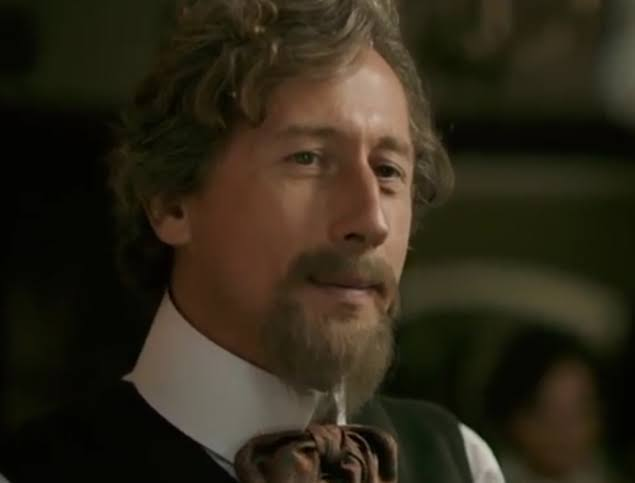
\includegraphics[scale=0.12, angle=-18]{Jost_Winteler.jpeg}
\caption{\textcolor{White}{Jost Winteler: Humanista y profundo. Totalmente opuesto a la rectitud de una institución.}}

\end{SCfigure}

\vspace{5cm}

\textcolor{Red}{\emph{(Aparte de las obviedades de Philipp Lenard o Fritz Haber)}}

\begin{SCfigure}

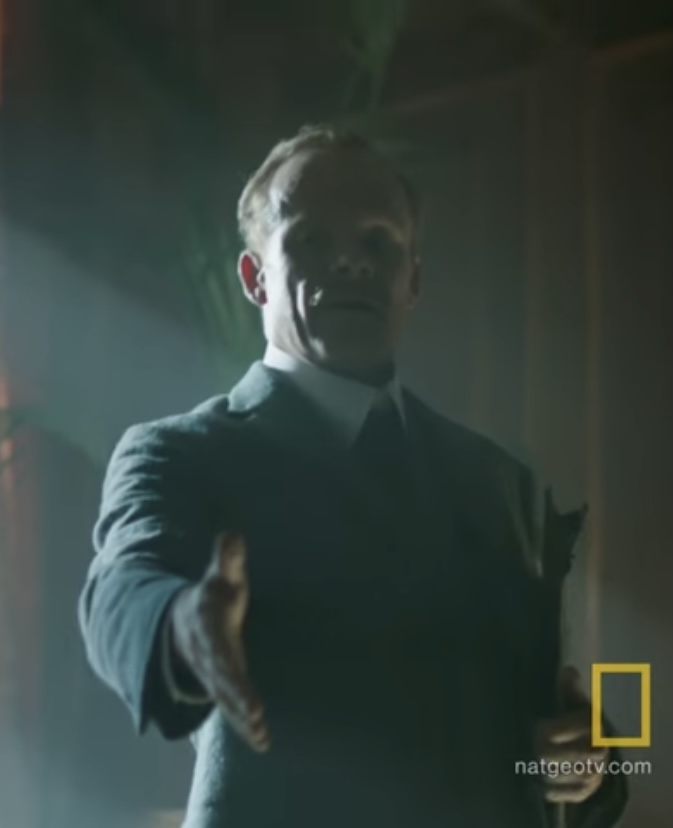
\includegraphics[scale=0.12, angle=8]{Friedrich_Weber.jpeg}
\caption{\textcolor{White}{Friedrich Weber: Profesor universitario recto y sistemático, bajo los estándares de Einstein «un mero especialista», todo lo contrario a Jost Winteler}}

\end{SCfigure}

\vspace{-10cm}

\marginnote{\tiny{Su conocimiento es su debilidad, y tu creatividad es tu fuerza.}}[3cm]

\fancyfoot[L]{}




\end{document}
